% assignment_1.text - Assignment 1 for Machine Learning class (Spring 2015)
% Chanmann Lim - February 2015

\documentclass[a4paper]{article}

\usepackage[margin=1 in]{geometry}
\usepackage{amsmath}
\usepackage{listings}
\usepackage{graphicx}
\usepackage[T1]{fontenc}

\everymath{\displaystyle}

\begin{document}
\setcounter{page}{8}
% \thispagestyle{empty}
% \pagestyle{empty}

\subsection*{4. }

%
% (1) Plot two histograms
%
\paragraph{(1) } Histogram of the Salman and Seabass lightness ~\\
\begin{figure}[h!]
  \centering
    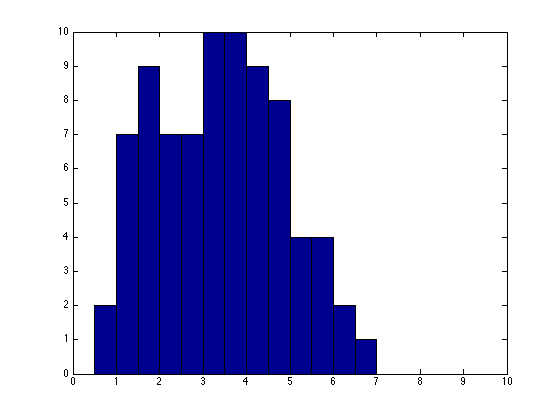
\includegraphics[scale=.6]{images/salmon_hist.png}
  \caption{Salmon lightness histogram}
\end{figure}

\begin{figure}[h!]
  \centering
    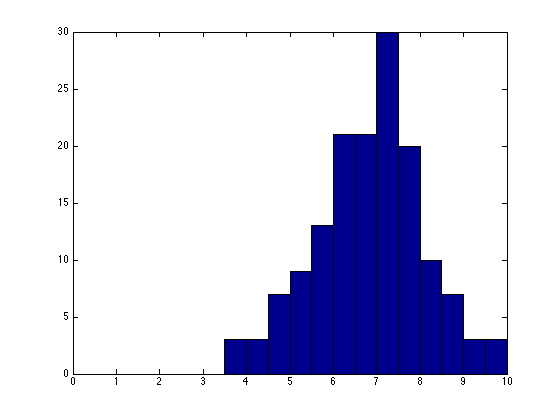
\includegraphics[scale=.6]{images/seabass_hist.png}
  \caption{Seabass lightness histogram}
\end{figure}

%
% (2) Find P(salmon) and P(seabass)
%
\paragraph{(2) } $P(salmon) = 0.34783$ and $P(seabass) = 0.65217$.

%
% (3) Plot P(lightness|salmon) and P(lightness|seabass)
%
\paragraph{(3) } Plots of $P(lightness|salmon)$ and $P(lightness|seabass)$ ~\\
\begin{figure}[h!]
  \centering
    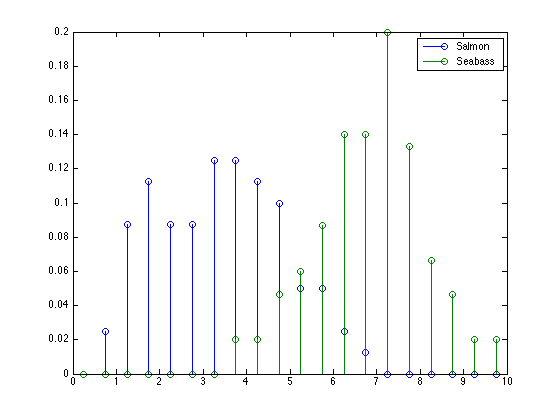
\includegraphics[scale=.6]{images/conditional_probability_pmfs.png}
  \caption{P(lightness|salmon) and P(lightness|Seabass)}
\end{figure}

%
% (4) Compute probabilities
%
\paragraph{(4) } Compute probabilities: ~\\

$P(lightness\le5|salmon) = 0.8625$ and $P(lightness\le8|salmon) = 1$ \\

$P(lightness\ge5|seabass) = 0.91333$ and $P(lightness\ge2|seabass) = 1$

%
% (5) Plot P(lightness)
%
\paragraph{(5) } Plot of the evidence pmf P(lightness) ~\\
\begin{figure}[h!]
  \centering
    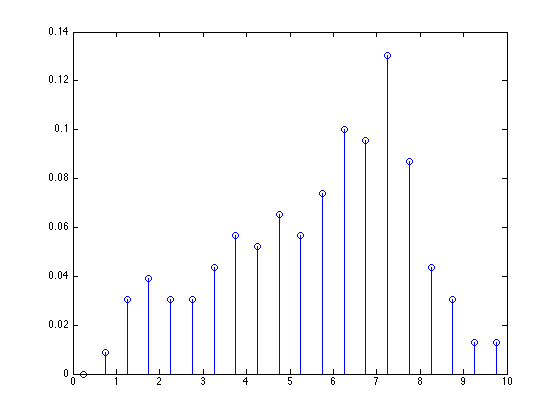
\includegraphics[scale=.6]{images/p_lightness.png}
  \caption{P(lightness)}
\end{figure}

%
% (6) Plot posterior probabilities
%
\paragraph{(6) } Plot the posterior probabilities $P(salmon|lightness)$ and $P(seabass|lightness)$ ~\\
\begin{figure}[h!]
  \centering
    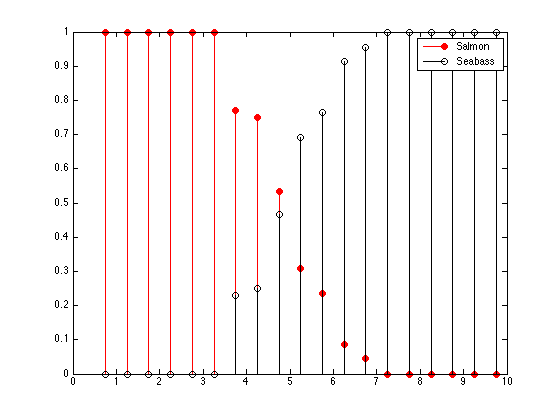
\includegraphics[scale=.6]{images/posterior_probabilities.png}
  \caption{Posterior probabilities}
\end{figure}

\newpage
\subsection*{Appendix:}
\lstinputlisting[language=Matlab, title=\lstname, basicstyle=\footnotesize]{assignment_1.m}

\end{document}